\clearpage
\subsection{Cursors}
\hrulefill

1. Create a Players Cursor and show the details of all the players.

\begin{lstlisting}[caption={ Query 1},label={lst:q-1}]
    DECLARE
    CURSOR player_cursor IS
    SELECT Player_ID, Player_Name, Player_Email
    FROM Player;
    p_info player_cursor%ROWTYPE;
BEGIN
    OPEN player_cursor;
    LOOP
        FETCH player_cursor INTO p_info;
        EXIT WHEN player_cursor%NOTFOUND;
        DBMS_OUTPUT.PUT_LINE('Player ID: ' || p_info.Player_ID);
        DBMS_OUTPUT.PUT_LINE('Player Name: ' || p_info.Player_Name);
        DBMS_OUTPUT.PUT_LINE('Player Email: ' || p_info.Player_Email);
    END LOOP;
    CLOSE player_cursor;
END;
/

\end{lstlisting}

\begin{figure}[H]
    \centering
    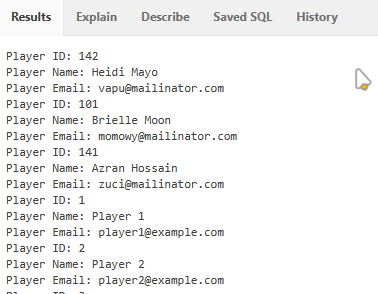
\includegraphics[width=0.5\textwidth]{images/plsql/cursor/Player Cursor.png}
    \caption{Result of Query 1}
\end{figure}

% retrieve the names and emails of all administrators 
2. Create an Admin Cursor and show the details of all the administrators.

\begin{lstlisting}[caption={ Query 2},label={lst:q-2}]
    DECLARE
    CURSOR admin_cursor IS
    SELECT Admin_Name, Admin_Email
    FROM Admin;
    
    admin_rec admin_cursor%ROWTYPE;
BEGIN
    OPEN admin_cursor;
    LOOP
        FETCH admin_cursor INTO admin_rec;
        EXIT WHEN admin_cursor%NOTFOUND;
        DBMS_OUTPUT.PUT_LINE('Admin Name: ' || admin_rec.Admin_Name);
        DBMS_OUTPUT.PUT_LINE('Admin Email: ' || admin_rec.Admin_Email);
    END LOOP;
    CLOSE admin_cursor;
END;
/
\end{lstlisting}
\clearpage
\begin{figure}[H]
    \centering
    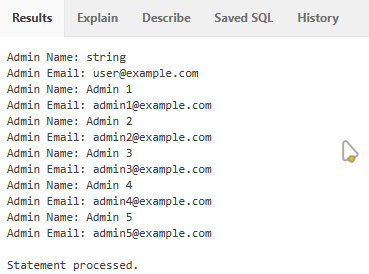
\includegraphics[width=0.5\textwidth]{images/plsql/cursor/Admin Cursor.png}
    \caption{Result of Query 2}
\end{figure}
% Organization Finance Cursor
3. Create an Organization Finance Cursor and show the details of all the organizations and their finances.

\begin{lstlisting}[caption={ Query 3},label={lst:q-3}]
    DECLARE
    CURSOR finance_cursor IS
    SELECT o.Organization_Name, f.Finance_Balance
    FROM Organization o
    JOIN Finance f ON o.Finance_ID = f.Finance_ID;
    fin_info finance_cursor%ROWTYPE;
BEGIN
    OPEN finance_cursor;
    LOOP
        FETCH finance_cursor INTO fin_info;
        EXIT WHEN finance_cursor%NOTFOUND;
        DBMS_OUTPUT.PUT_LINE('Organization Name: ' || fin_info.Organization_Name);
        DBMS_OUTPUT.PUT_LINE('Finance Balance: ' || fin_info.Finance_Balance);
    END LOOP;
    CLOSE finance_cursor;
END;
/
\end{lstlisting}
\begin{figure}[H]
    \centering
    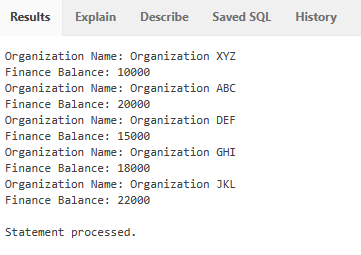
\includegraphics[width=0.5\textwidth]{images/plsql/cursor/Organization Finance Cursor.png}
    \caption{Result of Query 3}
\end{figure}